% ----------------------------------------------------------------------------------------\
% ---------------------------------------------------------------------------------------\
\subsection{Modificación de Probabilidades}
% ----------------------------------------------------------------------------------------\
% ---------------------------------------------------------------------------------------\

Recordemos el modelo original, donde las redes bayesianas son las encargadas de indagar en 
la satisfacción laboral y cuenta con tres variables clave:
\begin{itemize}
    \item[] $(a)$ Horas de trabajo $(H)$: \textit{largas, moderadas o cortas}.
    \item[] $(b)$ Balance trabajo-vida $(B)$: \textit{equilibrado o no equilibrado}.
    \item[] $(c)$ Satisfacción laboral $(S)$: \textit{satisfecho, neutral e insatisfecho}.
\end{itemize}


Cuando pensé en la modificación para esta parte del trabajo pensé en un cambio que he tenido
a lo largo de la carrera ya que cuando entre, pensaba que ir a la oficina a programar sería 
algo que me hiciera muy feliz, paso el tiempo y ahora sé que el cambio que me gustaría es 
trabajar desde casas. \\ 

Trabajar desde casa no es solo para programadores o trabajos que requieran estar detras de 
una computadora, pensé en pesonas del campo, más especificamente en un pastor quien tiene que 
ver que sus ovejas no sa vayan muy lejos y si esta se va, poder encontrarla rapidamente. Es 
así como pensé en un segundo parametro para esta tarea: ayuda de inteligencia artifical (IA). \\ 

Imaginemos que el pasor esta en una zona montañosa, aunque si debe estar con sus ovejas 
la ayuda de la inteligencia artifical podría ayudar con un dron que siga a sus ovejas y si 
una sale del limite, el dron la pueda seguir y decirle al pastor donde esta. \\ 

Basicamente las dos modificaciones que se tendrán contempladas serán las de un horario más 
flexible (trabajando desde casa) y el poder contar con herramientas con inteligencia artifical
que ayuden a terminar nuestras tareas dentro del trabajo.\\ 


% ---------------------------------------------------------------------------------------\
\subsubsection*{Horas de trabajo}
% ----------------------------------------------------------------------------------------\
La flexibilidad en horarios de trabajo permitido hacerlo desde casa con ayuda de la IA nos 
da una distribución más equilibrada de las horas de trabajo ya que se pueden cumplir en 
ciertos lapsos a lo largo del día o poder terminar mucho antes y no estar un una oficina.

\begin{itemize}
    \item Valores antes: [[0.6], [0.3], [0.1]] \textit{largas, moderadas o cortas}
    \item Valores ahora: [[0.08], [0.65], [0.27]] \textit{largas, moderadas o cortas}
\end{itemize}


% ---------------------------------------------------------------------------------------\
\subsubsection*{Balance trabajo-vida}
% ----------------------------------------------------------------------------------------\
Arriba mencionamos que un horario en casa y el contar con herramientas que le permitan hacer
su trabajo más rapido podría hacer que el trabajador termine antes sus actividades lo que 
le permitira aprovechar el tiempo para hacer otras actividades en su vida.

\begin{itemize}
    \item Valores antes: [[0.4, 0.7, 0.2], [0.6, 0.3, 0.8]] \textit{equilibrado o no equilibrado}.
    \item Valores ahora: [[0.5, 0.85, 0.88], [0.5, 0.15, 0.12]] \textit{equilibrado o no equilibrado}.
\end{itemize}

% ---------------------------------------------------------------------------------------\
\subsubsection*{Satisfacción laboral}
% ----------------------------------------------------------------------------------------\

\begin{itemize}
    \item Valores antes: [[0.8, 0.05], [0.15, 0.6], [0.05, 0.35]] \textit{satisfecho, neutral e insatisfecho}.
    \item Valores ahora: [[0.88, 0.55], [0.1, 0.35], [0.02, 0.1]] \textit{satisfecho, neutral e insatisfecho}.
\end{itemize}

Para un trabajador entonces poder terminar sus activades antes y poder estar en casa para ser 
más productivo en su vida (por supuesto que es el caso optimo) encontrando balance trabajo-vida podría 
llevar a una mayor satisfacción laboral en general.

% ----------------------------------------------------------------------------------------\
% ---------------------------------------------------------------------------------------\
\subsection{Resultados}
% ----------------------------------------------------------------------------------------\
% ---------------------------------------------------------------------------------------\

Actualizar los packetes para no tener problemas 
\begin{itemize}
    \item \texttt{pip install --upgrade jupyter ipywidgets}
    \item \texttt{pip install --upgrade pgmpy}
\end{itemize}


% ---------------------------------------------------------------------------------------\
\subsubsection*{Comparación}
% ----------------------------------------------------------------------------------------\

Estos son los resultados de la primera red 
\begin{center}
    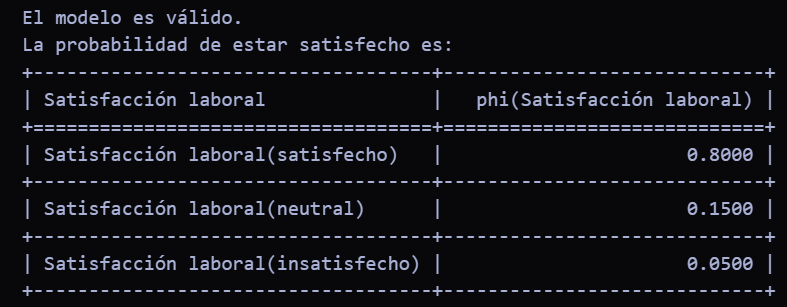
\includegraphics[scale = .6]{IMA/ejecucionRedBayesina.png}
\end{center}

Estos son los resultados de la red modificada 
\begin{center}
    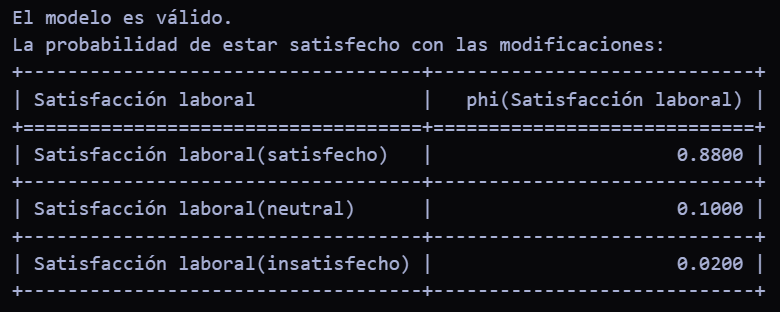
\includegraphics[scale = .6]{IMA/ejecucionRedModificada.png}
\end{center}
% ----------------------------------------------------------------------------------------\
Observamos como se ha incrementado $88\%$ la la satisfacción lo que nos dice que las condiciones 
nuevas para el trabajo tienen un impacto positivo en la vida de los empleados. Para la 
respuesas neutrales respecto a su satisfacción en el trabajo es baja $10\%$  lo que podemos 
decir que pocas personas se sentiran en las mismas situciones con los dos cambios realizados, 
mientras que con un $2\%$ la probabilidad de insatisfacción es muy baja lo cual dice que las 
personas les gusta más poder tener un horario flexible desde casa y tener ayuda de la 
tecnología.

% ----------------------------------------------------------------------------------------\
% ---------------------------------------------------------------------------------------\
\subsection{Modificación de Probabilidades}
% ----------------------------------------------------------------------------------------\
% ---------------------------------------------------------------------------------------\